\documentclass[11pt,a4paper,twoside]{article}

% LaTeX-Umsetzung der "Richtlinien f�r Projekt- und Diplomarbeiten"
% der LFE Medieninformatik, LMU M�nchen. (Autor: Richard Atterer, 27.9.2006, 23.10.2007), Bug-Fixing Mark Kaczkowski (23.6.2008)

\usepackage[T1]{fontenc} % sonst geht \hyphenation nicht mit Umlauten
\usepackage[latin1]{inputenc} % man kann schreiben ����, statt "a"o"u"s
%\usepackage[utf8]{inputenc} % wie oben, aber UTF-8 als Encoding statt ISO-8859-1 (latin1)
\usepackage[ngerman,english]{babel} % deutsche Trennregeln, "Inhaltsverzeichnis" etc.
%\usepackage{ngerman} % Alternative zum Babel-Paket oben
\usepackage{mathptmx} % Times-Roman-Schrift (auch f�r mathematische Formeln)

% Zum Setzen von URLs
\usepackage{color}
\definecolor{darkred}{rgb}{.25,0,0}
\definecolor{darkgreen}{rgb}{0,.2,0}
\definecolor{darkmagenta}{rgb}{.2,0,.2}
\definecolor{darkcyan}{rgb}{0,.15,.15}
\usepackage[plainpages=false,bookmarks=true,bookmarksopen=true,colorlinks=false,
  linkcolor=darkred,citecolor=darkgreen,filecolor=darkmagenta,
  menucolor=darkred,urlcolor=darkcyan]{hyperref}

% pdflatex: Bilder in den Formaten .jpeg, .png und .pdf
% latex: Bilder im .eps-Format
\usepackage{graphicx}

\usepackage[sorting=none, backend=biber, urldate=long]{biblatex}
\addbibresource{PursuitsInVr.bib}

 \usepackage{amsmath}
\usepackage{fancyhdr} % Positionierung der Seitenzahlen
\fancyhead[LE,RO,LO,RE]{}
\fancyfoot[CE,CO,RE,LO]{}
\fancyfoot[LE,RO]{\Roman{page}}
\renewcommand{\headrulewidth}{0pt}
\setlength{\headheight}{13.6pt} % behebt headheight Warning

% Korrektes Format f�r Nummerierung von Abbildungen (figure) und
% Tabellen (table): <Kapitelnummer>.<Abbildungsnummer>
\makeatletter
\@addtoreset{figure}{section}
\renewcommand{\thefigure}{\thesection.\arabic{figure}}
\@addtoreset{table}{section}
\renewcommand{\thetable}{\thesection.\arabic{table}}

\makeatother

\sloppy % Damit LaTeX nicht so viel �ber "overfull hbox" u.�. meckert

% R�nder
\addtolength{\topmargin}{-16mm}
\setlength{\oddsidemargin}{25mm}
\setlength{\evensidemargin}{35mm}
\addtolength{\oddsidemargin}{-1in}
\addtolength{\evensidemargin}{-1in}
\setlength{\textwidth}{15cm}
\addtolength{\textheight}{34mm}
%______________________________________________________________________

\begin{document}

\pagestyle{empty} % Vorerst keine Seitenzahlen
\pagenumbering{alph} % Unsichtbare alphabetische Nummerierung

\begin{center}
\textsc{Ludwig-Maximilians-Universit�t M�nchen}\\
Department ``Institut f�r Informatik''\\
Lehr- und Forschungseinheit Medieninformatik\\
Prof.\ Dr.\ Heinrich Hu�mann

\vspace{5cm}
{\large\textbf{Masterarbeit}}\vspace{.5cm}

{\LARGE The Use of Pursuits in Virtual Reality}\vspace{1cm}

{\large Carl Oechsner}\\\href{mailto:oechsner.carl@gmail.com}{oechsner.carl@gmail.com}

\end{center}
\vfill

\begin{tabular}{ll}
Bearbeitungszeitraum: & 1. 11. 2016 bis 1. 6. 2017\\
Betreuer: & Mohamed Khamis\\
%Externer Betreuer: & Manfred Manager\\
Verantw. Hochschullehrer: & Prof. Butz ODER Prof. Hu�mann
\end{tabular}
%______________________________________________________________________

\clearpage
\section*{Zusammenfassung}

Kurzzusammenfassung der Arbeit, maximal 250 W�rter.

\selectlanguage{english}
\section*{Abstract}

Short abstract of the work, maximum of 250 words.

\selectlanguage{ngerman}
\clearpage
\section*{Task}

Kopie der Original-Aufgabenstellung

\section*{Motivation}

Keine.

\vfill % Sorgt daf�r, dass das Folgende an das Seitenende rutscht

\noindent Ich erkl�re hiermit, dass ich die vorliegende Arbeit
selbstst�ndig angefertigt, alle Zitate als solche kenntlich gemacht
sowie alle benutzten Quellen und Hilfsmittel angegeben habe.

\bigskip\noindent M�nchen, \today

\vspace{4ex}\noindent\makebox[7cm]{\dotfill}

%______________________________________________________________________

\cleardoublepage
\pagestyle{fancy}
\pagenumbering{roman} % R�mische Seitenzahlen
\setcounter{page}{1}

% Inhaltsverzeichnis erzeugen
\tableofcontents

%Abbildungsverzeichnis erzeugen - normalerweise nicht n�tig
%\cleardoublepage
%\listoffigures
%______________________________________________________________________

\cleardoublepage

% Arabische Seitenzahlen
\pagenumbering{arabic}
\setcounter{page}{1}
% Ge�ndertes Format f�r Seitenr�nder, arabische Seitenzahlen
\fancyhead[LE,RO]{\rightmark}
\fancyhead[LO,RE]{\leftmark}
\fancyfoot[LE,RO]{\thepage}

\selectlanguage{english}

\section{Introduction}


%______________________________________________________________________

% Der Befehl \cleardoublepage erscheint nur vor \section, nicht vor
% den "kleineren" Gliederungsbefehlen wie \subsection!
\cleardoublepage % Neue rechte Seite anfangen
\section{Conceptual Framework}


\subsection{Eye Tracking}
\subsubsection{Pursuits}
- Papers on Pursuits, Orbits, and where they got cited

\subsection{Virtual Reality}
- mention Fove
- find papers in this direction
- more generally:  interaction in virtual reality and scenarios in which eye-tracking was used until now, its drawbacks and benefits and how vr applications could benefit from it

\subsection{Eye-based interaction in VR} 

\cleardoublepage
\section{Design Space}
\subsection{User Bound Objects}
\subsection{World Bound Objects}

\cleardoublepage
\section{Implementation}
\label{Implementation}

\subsection{Communication with the Eye Tracker}

\subsection{Interpretation of Gaze Data using Pursuits}

\subsection{Measurement of the Field of View Wearing a Virtual Reality Headset}
\label{fovMeasure}

In order to report sizes and distances investigated in the main study, a method was needed to transform Unity units into visual degrees. In conventional eye-tracking studies that involve interaction with a screen, the person is positioned in a spot at a certain distance to the screen. Using this distance, the size and the resolution of the screen, visual angles can be calculated for the displayed objects. But due to different skull shapes the distance between the eyes and Vive lenses varies from person to person. Therefore an object with a certain size has varying values in visual degrees. At the beginning of each study session the participant was shown a Unity scene in which the individual values for the total available horizontal and vertical field of view were measured and matched to the corresponding pixel values.

First a horizontal scale is displayed that consists of 360 lines evenly distributed on an XZ-plane around the user's head in the virtual environment. Every five lines the corresponding value is displayed so that the participants can tell it to the experimenter. All scale elements are child elements of the virtual Vive camera in Unity so that the scale moves in the same manner as the user's head and its position in relation to the user's eyes remains constant. The scale is then rotated around the y-Axis so that eventually the line denoted with zero degrees meets the left edge of the screen area the user can perceive through the lenses. Now the user is asked to read the value off the scale at the very right of his field of view which constitutes the horizontal field of view the user has wearing the headset (see Fig. \ref{horScale}). In the same manner the vertical FOV is determined.

Subsequently it is determined to which pixel values the minima and maxima of the field of view correspond to. This is simply done by moving a vertical red line in front of the user until it meets the left and right edges of the available field of view and by recording the corresponding x-values in pixels. Accordingly the same procedure is performed with a horizontal line for acquiring the individual y-values. Given these six values, sizes, positions and distances can be calculated using the Law of Tangens (see Fig. \ref{fieldOfViewGraphic}) and Equation \ref{lambdaequations}):

\begin{figure}
	\centering
	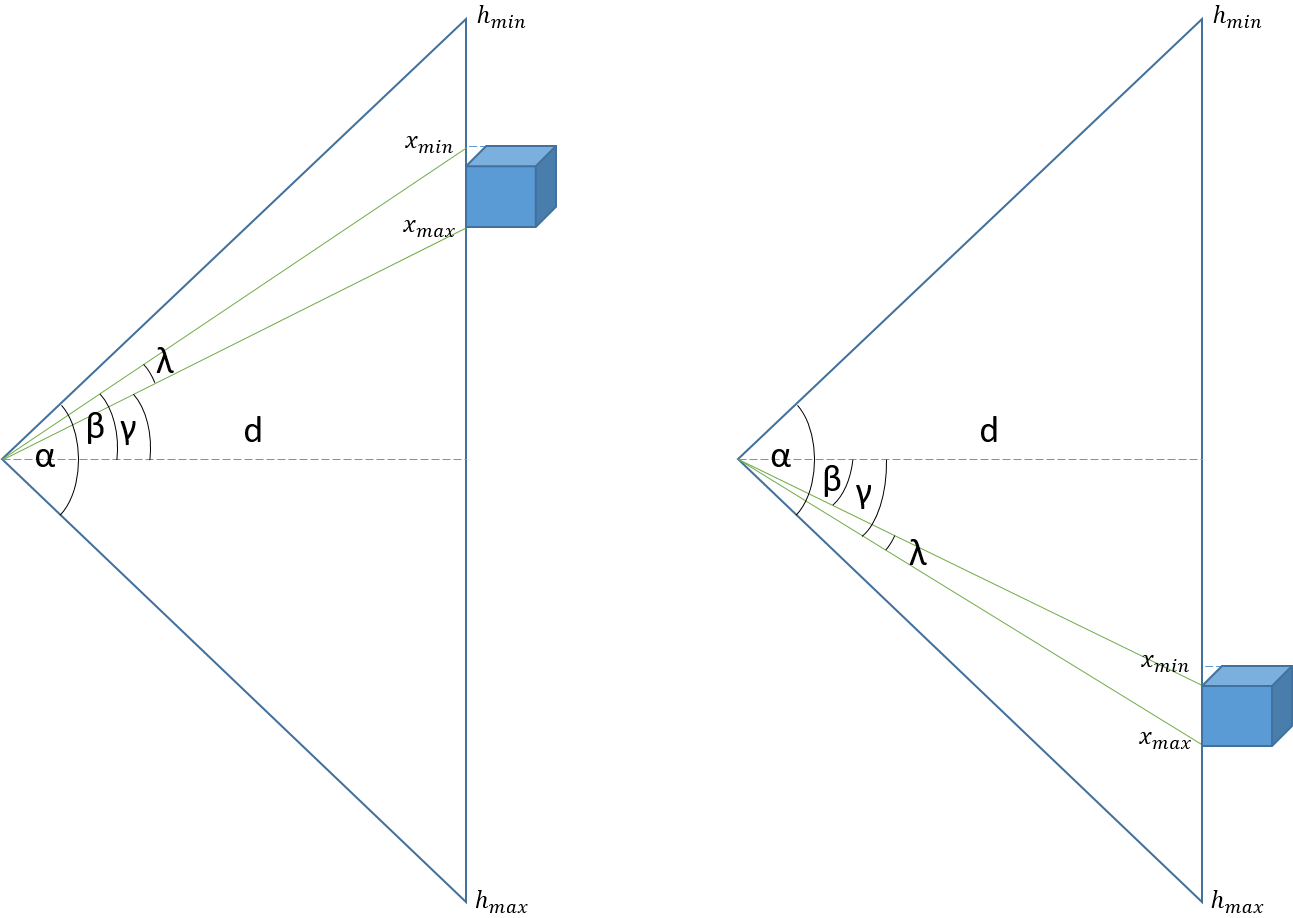
\includegraphics[height=8cm]{FOV1.png}
	
	\caption{Model used for the calculation of the horizontal size of a displayed object in visual degrees. $\alpha$: horizontal FOV, $\beta$: angle between the object's left edge and the horizontal center, $\gamma$: angle between the object's right edge and the horizontal center, $\lambda$: visual angle that the object occupies in the user's FOV, $x_{min}$: minimum x-value of the object in pixels, $x_{max}$: maximum x-value of the object in pixels, $d$: distance eye to screen, $h_{min}$: left edge of the FOV in pixels, $h_{max}$: right edge of the FOV in pixels. See \ref{lambdaequations}}
	
	\label{fieldOfViewGraphic}
\end{figure}

\begin{figure}
\begin{equation}
	d=\frac{W}{\tan\left(\frac{\alpha}{2}\right)}
\end{equation}

\begin{equation}
\beta = \arctan \left( \frac{\left| x_{min} - \frac{W}{2} \right|}{d} \right)
\end{equation}

\begin{equation}
\gamma = \arctan \left( \frac{\left| x_{max} - \frac{W}{2} \right|}{d} \right)
\end{equation}

\begin{equation}
\lambda =
\begin{cases}
\beta - \gamma &\mbox{if } x_{min} < \frac{W}{2} \land x_{max} < \frac{W}{2} \\
\beta &\mbox{if }  x_{min} < \frac{W}{2} \land x_{max} \equiv \frac{W}{2} \\
\beta + \gamma &\mbox{if }  x_{min} < \frac{W}{2} \land x_{max} > \frac{W}{2} \\
0 &\mbox{if }  x_{min} \equiv \frac{W}{2} \land x_{max} \equiv \frac{W}{2} \\
\gamma &\mbox{if }  x_{min} \equiv \frac{W}{2} \land x_{max} > \frac{W}{2} \\
- \beta + \gamma &\mbox{if }  x_{min} > \frac{W}{2} \land x_{max} > \frac{W}{2}
\end{cases}
\end{equation}

\caption[Equation]{For better readability $ W = \frac{h_{max}-h_{min}}{2} $ applies to equations 1 to 4. $\alpha$: horizontal FOV, $\beta$: angle between the object's left edge and the horizontal center, $\gamma$: angle between the object's right edge and the horizontal center, $\lambda$: visual angle that the object occupies in the user's FOV, $x_{min}$: minimum x-value of the object in pixels, $x_{max}$: maximum x-value of the object in pixels, $d$: distance eye to screen, $h_{min}$: left edge of the FOV in pixels, $h_{max}$: right edge of the FOV in pixels.}
\label{lambdaequations}
\end{figure}

\begin{figure}
	\centering
	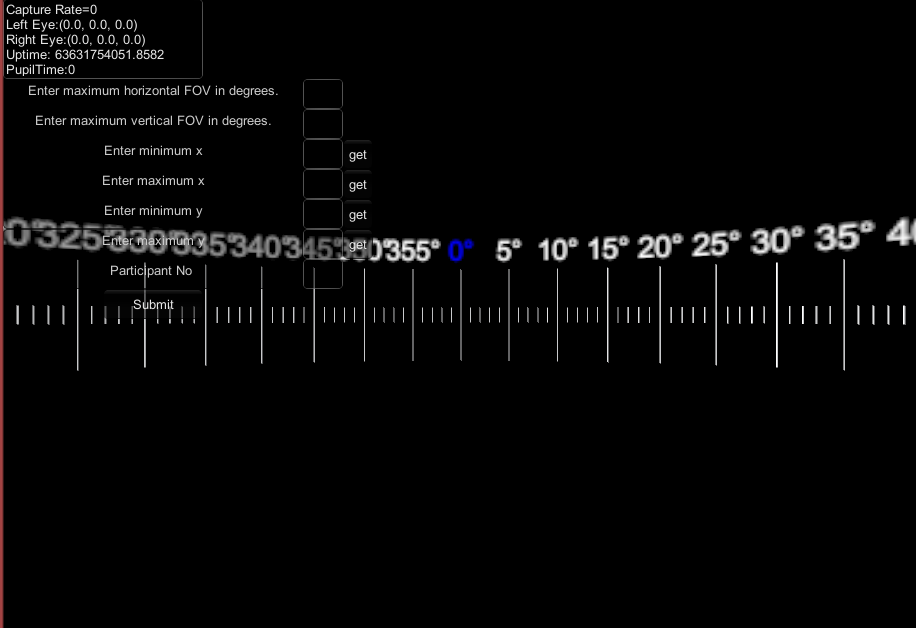
\includegraphics[height=6cm]{FOV2.png}
	\caption{Horizontal scale that was presented to the users in order to determine their horizontal FOV}
	\label{horScale}
\end{figure}

\cleardoublepage
\section{Evaluation}

\subsection{Trial Study}
The system described in \ref{Implementation} is able to detect fixation on any user-bound object that is moving within a scene in Unity. Objects and their trajectories can have any shape, size or velocity. The trial study had several purposes: First, to identify a manageable set of independent variables that can be further investigated in the main study. Second, to exclude certain settings which don't work and there don't need to be investigated. Third, to find parameters for the correlation procedure that result in reliable results. The trial study was conducted with 14 participants. Measurements are indicated in Unity units which was changed in the main study using the procedure described in \ref{fovMeasure}. One Unity unit corresponds to one meter in ``real-world units''. Objects moving on trajectories referred to as ``horizontal'' only alter the x component and objects on ``vertical'' trajectories only alter the y component of their local position respectively. In both cases the objects moved along the whole available visual range, i.e. along an trajectory with a length of 6 units.

\subsubsection{Setting}
 The virtual objects were decided to be numbered cubes to easily tell the participants where to fixate on. All objects were located on a plane that was orthogonal to the camera's z-Axis and located at a distance of 6.78 units in front of the camera. The available visible space was determined empirically and reached from -3 to 3 units both horizontally and vertically on this very plane. When a fixation was detected by the software, an object was highlighted with a halo effect. There were several scenes created to investigate four different variables. In the following enumeration the scene is referenced with its number and the independent variable that was focussed on.

\begin{description}	
	\item [Scene 1a | \textit{Number}:] A cube with an edge length of 0.7 units was moving back and forth on a horizontal trajectory that ranged from one edge of the visible space to the other thus having a length of 6 units. To determine up to which number the system can correctly differentiate which object is selected, $\left\lbrace 3,5,7,9\right\rbrace $ cubes were shown at the same time. At each increase of the number of displayed objects, two trajectories were added at the top and the bottom of the existing ones. Each cube started moving from a random position on its trajectory. The trajectories had a vertical distance of 0.7 units to each other so that the cubes don't overlap. As the Pursuits approach would not work if all objects had the same velocity, they were all moving with unique speeds. The minimum difference between two speed values was 0.2 units per second.
	
	\item [Scene 1b | \textit{Number}:]
	Additionally, circular trajectories were investigated. $\left\lbrace2,3,5\right\rbrace $ numbered cubes were moving clockwise along a radial path on the aforementioned orthogonal plane with a radius of 2 units and a velocity of $ 45 \frac{�}{s} $.
	
	\item [Scene 2a | \textit{Position}:] In this scene three objects were shown at a time at the edges of the visible area to determine if the object position has an impact on tracking performance. The objects moved along horizontal trajectories and were positioned either at the top or at the bottom of the field of view. The vertical difference between them was 1 unit with the outermost trajectory positioned at +/- FIND OUT VALUE!!. The objects started at random positions along the trajectory and had unique velocities with FIND OUT VALUES!!! differences.
	
	\item [Scene 2b | \textit{Position}:]
	  Three objects on vertical trajectories were positioned at the left or at the right edges of the FOV. The trajectories always had a distance of 1 unit to each other with the outermost trajectory positioned at FIND OUT VALUE!!!. The velocity delta was 0.4 units per second to make differentiation possible.
	
	\item [Scene 3 | \textit{Size}:]: Cubes of three different sizes were compared to each other in terms of fixation detection. Three cubes were displayed at a time on horizontal trajectories with an edge length of \{0.3,1.5\} units to compare them to the standard 0.7 unit cubes. Their trajectories had a distance of one unit in the small and 2.5 units in the large case to prevent overlapping. Their velocities differed by one unit per second.
	
	\item [Scene 4 | \textit{Trajectory Shape}]: Three different trajectory shapes \{horizontal, vertical, circular\} are compared to each other within one scene each being equipped by a 0.7 unit cube. The linear trajectories had a length of 6 units and a speed of 2 units per second, the circular trajectory had a radius of 2 units and a speed of 45 degrees per second. 
\end{description}

\subsubsection{Procedure}
At the beginning, each participant was shown how to put on the headset. Then, on the experimentee's head, it was adjusted in a way that it was attached safely but not too tightly to their head using the three Velcro fasteners of the Vive's harness. Being showed each scene the participants were asked to fixate on a certain object with their eyes by naming its digit which was documented in a Google Spreadsheet. The experimenter then controlled visually if the mentioned cube was being highlighted. If highlighting of an object was not constant or not given at all, detection quality was tried to improve by manipulating the values for the correlation process. HOW WAS THIS DONE? After each setting the users were asked which characteristics they found most convenient and represented best what they were looking at. The answers and other remarks were documented in a Google Spreadsheet.

\subsubsection{Results and Discussion}
\label{correlator}
During the course of the trial study, most reliable results were achieved with a Pearson threshold of 0.4, a correlation frequency of 3.33, a correlation time window of 300ms and a correlation averaging window of 900 milliseconds meaning that the average of the three last coefficients for an object was compared to the threshold (also see chapter \ref{Implementation}).

All participants but one preferred circular over linear trajectories, because they were more convenient to follow. One participant mentioned that this was due to the larger distance between the objects. Furthermore, all but one person preferred smaller cubes over large cubes. Most of them agreed on them being easier to follow and to focus on. When it came to the objects' positions many agreed that differences between top and bottom (respectively left and right) were hard to tell. When they had to decide which position was more convenient, there was no discernible tendency except least users voted for the upper position. Regarding the number of objects, most experimentees preferred no more than five objects. As for the linear trajectories this was to the perceived drop in detection performance. Because there were hardly any detection errors with five objects on a circular trajectory three more cubes were shown additionally moving counter-clockwise to sound out the limits of this setting. Although detection was still fairly reliable most agreed on a limit of five objects due to visual clutter.

As there was visual feedback on the selection provided the participants knew if a selection was right or wrong. If the software detected fixations in one setting better than in another this might have had an influence on their opinion. 
% cubes, numbers, find flaws in the framework, optimize logging for a straightforward analysis process, object size and trajectory size should be considered separately and have a certain ratio, users prefer a limited area they can fixate their eyes on

\subsection{Main Study}

The main study had two primary goals: First, to find design guidelines for traceable objects in a virtual reality setting employing Pursuits. Second, by adding a task in which the user is moving within the VR area, to figure out to which amount pursuing objects is possible while performing another task. The Correlator settings found credible in \ref{correlator} were used throughout the main study. It consisted of two parts:

\begin{enumerate}
	\item \textbf{Abstract Scenarios:} For evaluating the quality of the employed detection algorithm participants had to fixate certain objects in a low-stimulus virtual environment, once while being seated, once while moving (see \ref{abstractScene}).
	\item \textbf{Use Case Scenarios:} Two scenarios were created to demonstrate and investigate the developed interaction technique in different use cases (see \ref{useCaseScene}).
\end{enumerate}

Before each session, the field of view of each participant was measured using the method described in section \ref{fovMeasure}.

\subsubsection{Abstract Scenario}
\label{abstractScene}

In the abstract scenario we aimed for investigating certain variables in an isolated manner to acquire quantitative data for further analysis. There should be no biasing clues or embellishments distracting participants from their task and to make sure the observed effects are solely due to manipulations of the independent variables. For this reason, Chaperone bounds visualization was disabled and the Unity Camera Clear Flags were set to solid black, resulting all screen parts but the cubes to be coloured black. As the relative size of an object is a monocular depth clue, a script was used to ensure objects always have the same absolute size to the viewer, i.e. the object will be down-scaled when it moves towards the viewer (decreasing z-Value) and up-scaled when it moves away (increasing z-Value) \cite{Goldstein2002}. Another key difference to the Use Case Scenario is that no feedback is provided if or which object is detected, which might have an impact on subjective ratings.

After each of the two scenes, participants had to answer a questionnaire Additionally every participant filled in a NASA-TLX questionnaire without pair-wise comparisons either in English or  German to measure the perceived workload while performing the respective tasks \cite{Hart2006} \cite{tlxger} \cite{tlxeng}. This was done once after each of the two scenes. As neither \textit{object velocity} and \textit{position} had a mentionable effect and circular \textit{trajectories} were rated both most reliable and comfortable to use in the trial study, these variables were decided to be fixed throughout the main study. Furthermore, as detection was rated most agreeable with up to five objects, this was the final choice for the number of objects per trajectory.

\begin{itemize}
	\item \textbf{Independent variables}: Trajectory radius \{0.5, 1.5, 2.5\}, Object size \{0.3, 0.65, 0.9\}, Object Depth \{2, 6, 16\}, User is moving \{yes, no\}
	\item \textbf{Dependent variables}: Selection time [s], error rate \{correct, not correct\}
	\item \textbf{Fixed variables}: Object velocity \{45 �/s\}, position \{center\}, trajectory shape \{circular\}, Nr of objects per trajectory \{5\}
\end{itemize}


\subsubsection*{Static User}

The seated user is shown every combination of size, radius and depth in a black surrounding in a randomized order. There are five coloured cubes of the same size moving along one circular trajectory. One cube is randomly chosen to be coloured red, the other four ones are coloured blue. Before each trial the user is told to fixate on the red cube. A cube counts as selected as soon as its coefficient is greater than the others' and exceeds the threshold. The procedure for calculating the threshold is described in section \ref{Implementation}. For identification purposes the cubes are numbered and have their respective number as a black digit texture appearing on each of their faces. It counts as an error if a blue cube or nothing is selected. The trajectory centre is in the centre of the participant's field of view. The objects appear and start moving when the experimenter presses the space bar. The objects disappear as soon as a cube is selected.

\subsubsection*{Moving User}

In this scenario the experimentee is exposed to the same 27 combinations of radius, size and depth. To evaluate selection performance while the user is moving, the participant is told to perform a simple walking task. A white square on the floor indicates where the user is supposed to go. The square alternately appear in the middle of two opposing borders of the virtual play area. For safety purposes Chaperone bounds were enabled in this scenario. Additionally the participants were told to walk up to the bounds and to familiarize with them by feeling for the walls in the real environment. Time and error rate measurements are performed in the same way as in the static task.

In the original study design, the white square appeared in random locations within the play area. After some trials it appeared that the process of searching end re-orientating was much too demanding and resulted in feeling overwhelmed and in 


\subsubsection{Use Case Scenario}
\label{useCaseScene}

Besides the Abstract Scenario we wanted to examine the applicability of Pursuits in concrete use cases. There were two scenes created: one in which participants are required to be moving and one in which they are not. In both scenarios users had to fixate on objects moving along a circular trajectory to trigger certain actions in order to achieve a goal. The participant is provided input feedback on the correctness of the selected object. At the end of each setting qualitative feedback is gathered with both a NASA-TLX questionnaire and a User Experience Questionnaire (UEQ). The latter was employed to ascertain the overall impression the users received of the presented interaction technique . The UEQ is broadly used e.g. in evaluations on user satisfaction or quality assurance during software development. It consists of 26 scales in form of a seven grade semantic differential \cite{Laugwitz2009} \cite{Hinderks}. 

\subsubsection*{Static User}
The experimentee is asked to walk up to a virtual ATM machine and enter a PIN that is given to them by the experimenter. A number can be entered by looking at a cube tagged with the respective digit. The numbers one to five are moving along one circular trajectory in a clockwise manner, the numbers five to nine and zero are moving on a second trajectory in a counter-clockwise manner. There is a counter for every cube that is increased whenever the software detects a fixation (just like in the abstract setting). After a time limit ${t}_{s}\in \{0.3,0.5,0.7,0.9\}$ TO BE DETERMINED!! the cube with the highest counter is considered as input. Every time an input is accepted, the user gets visual feedback in form of a temporal highlighting of all cubes so it is clear that they can move on to the next number.

\subsubsection*{Moving User}

For the moving user task we decided on a game setting in which the user is asked to ``shoot'' at meteors that move into the field of view. Like in the abstract case the target object is coloured red while the other objects are coloured blue. There is only one target object visible at a time to clearly detect wrong selections. The positions and shapes of the object trajectories are randomly chosen by the software.

\subsubsection{Objective Results}
Statistics from the measured Data of the Abstract Scenario

\subsubsection{Subjective Results}
Results from NASA TLX, UEQ and additional questions of the participant form.


	

\begin{table}[h]
\begin{center}
\begin{tabular}{|c|c|c|c|}
	\hline 
	\multicolumn{2}{|c|}{\textbf{Abstract Scenario}} &  \multicolumn{2}{c|}{\textbf{Use Case Scenario}} \\ 
	\hline 
	Stationary & Walking & Stationary & Walking \\ 
	\hline 
	21.08 & 36.38 & 47.13 & 47.27 \\ 
	\hline 
\end{tabular} 
\end{center}
\caption{Averages of the Overall Rating Score measured for all participants after the respective Scenario}
\label{MainStudyTLX}
\end{table}

\subsubsection{Discussion}

\subsection{Follow-Up Study}
To differentiate between the effects of radius and velocity a Follow-Up study was conducted. Here its results and the assumptions drawn from it. Of course, due to the small sample size, further investigations have to be carried out on this matter to prove the assumptions.

\subsubsection{Results and Discussion}

\cleardoublepage
\section{Conclusion}

\cleardoublepage
\section{Limitations and Future Work}

Limitations: 

Quality of Tracking Data relies on the eyes being in focus. As the cameras' focus can only be adjusted manually the headset has to be put on and off the head every time an adjustment has to be made. Due to the short distance it happened that even if pupils were in focus when looking straight, they might get blurry if the eyes move to fixate an object at the edge of the field of view. This might have had an influence on the tracking performance measured for large radii.

Measuring the field of view relied on the participants interpreting the presented scale correctly

It lies in the nature of gaze data that it is calibrated and fits only to one user perfectly. The presented system also works with other users using the same calibration but performance might vary between users.

%\begin{figure}%[btph]
  %% Datei ``beispielbild.eps'' oder ``beispielbild.png'', zentriert
  %\begin{center}\includegraphics{beispielbild}\end{center}

  %% Datei auf 8cm Breite verkleinert/vergr��ert
  %\includegraphics[width=8cm]{beispielbild}
  %% Datei auf ganze Breite des Texts vergr��ert
  %\includegraphics[width=\columnwidth]{beispielbild}
  %% Datei auf 60% der Textbreite verkleinert/vergr��ert
  %\includegraphics[width=.6\columnwidth]{beispielbild}
  %% Weitere Optionen (Ausschnitt, drehen etc.) in der Doku zum graphicx-Paket

%  \begin{center}\LARGE [BILD]\end{center}
%  \caption{Bildunterschrift}
%  \label{fig:beispielbild}
%\end{figure}


%Siehe Abbildung \ref{fig:beispielbild} oder einschl�gige Literatur, z.B.
%\cite[Seite 6]{Ivory01} oder \cite{NielsenAlertbox}.
%
%\bigskip % Gr��erer Abstand zum vorherigen Absatz
%\textbf{Hinweis:} Die Verweise im generierten PDF (HTTP-Links, Verweise auf Kapitel oder Bilder) sind leicht eingef�rbt. Wer das nicht will, z.B. weil es die Druckkosten erh�ht, kann am Anfang des Dokuments \texttt{linkcolor} usw. auf ``black'' setzen.


%\subsection{Medien}
%
%\begin{figure}
%  \begin{center}\LARGE [BILD]\end{center}
%  \caption{Noch ein Bild}
%  \label{fig:beispielbild2}
%\end{figure}
%
%\begin{itemize}
%  \item Gesellschaftliche Medien
%  \item Technische Medien
%\end{itemize}
%
%
%\subsection{Informatik}
%
%
%\subsection{Medieninformatik}
%
%\begin{description}
%  \item[Medienwirkung:] Ein Spezialfach der Kommunikationswissenschaft. F�r das erfolgreiche Studium des Anwendungsfachs Mediengestaltung ist eine k�nstlerische Begabung erforderlich.
%  \item[Medienwirtschaft:] Ein Spezialfach der Betriebswirtschaftslehre
%  \item[Mediengestaltung:] Ein Spezialfach der Kunstwissenschaft
%\end{description}
%
%\subsubsection{Was Sie schon immer wissen wollten, aber nie zu fragen
%  wagten}
%
%\paragraph{�berschrift}
%Diese �berschrift erscheint fettgedruckt am Anfang des Absatzes. \cite{NielsenAlertbox}
%
%\subsubsection{Was Sie nicht wissen wollten}
%
%Text text textextext\footnote{Oder so �hnlich}.

%\_____________________________________________________________________

\cleardoublepage
%\section{Zusammenfassung}
%
%\begin{figure}
%  \begin{center}\LARGE [BILD]\end{center}
%  \caption{Bild}
%  \label{fig:beispielbild3}
%\end{figure}
%______________________________________________________________________

\cleardoublepage
\fancyhead[LE,RO,LO,RE]{} % Keine Kopfzeile mehr oben auf jeder Seite
\section*{DVD Contents}
%______________________________________________________________________

\cleardoublepage
\printbibliography[title={Literature}, nottype=online]
%\bibitem{Ivory01}
%
%  M.\ Y.\ Ivory, M.\ Hearts:
%  \href{http://www.ischool.washington.edu/myivory/thesis/thesis.pdf}{%
%    An Empirical Foundation for Automated Web Interface Evaluation}.
%  Ph.D. thesis, University of California at Berkeley, 2001


\cleardoublepage
\printbibliography[title={Web-References}, type=online]
%\bibitem{NielsenAlertbox}
%
%  J.\ Nielsen: Alertbox: Current Issues in Web Usability
%  \url{http://useit.com/alertbox/}, accessed April~24, 2005.


\end{document}
